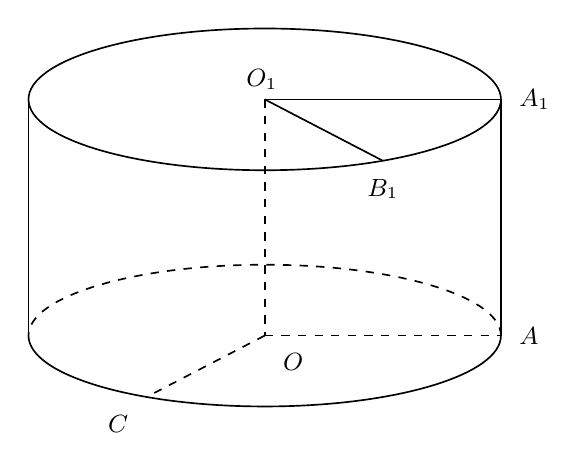
\begin{tikzpicture}[line width=.6pt, font=\small]
\coordinate (O1) at (0,3);
\coordinate (O) at (0,0);
\coordinate (A1) at (3,3);
\coordinate (A) at (3,0);
\coordinate (B1) at (1.5000000000,2.2205771366);
\coordinate (C) at (-1.5000000000,-0.7794228634);
% top rim fully visible
\draw (O1) ellipse (3 and 0.9);
% bottom rim: back hidden dashed, front visible solid
\draw[dashed] (3,0) arc [x radius=3, y radius=0.9, start angle=0, end angle=180];
\draw (-3,0) arc [x radius=3, y radius=0.9, start angle=180, end angle=360];
% lateral generatrices
\draw (-3,3) -- (-3,0);
\draw (3,3) -- (3,0);
% axis
\draw[dashed] (O1) -- (O);
% radii
\draw (O1) -- (A1);
\draw[dashed] (O) -- (A);
\draw[dashed] (O) -- (C);
\draw (O1) -- (B1);
% labels offset from strokes
\node[above=3pt,xshift=-1.0pt,yshift=-3.0pt] at (O1) {$O_{1}$};
\node[right=3pt] at (A1) {$A_{1}$};
\node[below=3pt] at (B1) {$B_{1}$};
\node[below right=3pt] at (O) {$O$};
\node[right=3pt] at (A) {$A$};
\node[below left=3pt] at (C) {$C$};
\end{tikzpicture}
